\section{Dynamic Programming}

\subsection{Rucksack-Problem}
Gegeben:
\begin{itemize}
    \item n Gegenstände mit einem bestimmten Gewicht und Wert
    \item Rucksack mit einer bestimmten Gewichts-Kapazität
\end{itemize}
Gesucht:
\begin{itemize}
    \item Füllung des Rucksacks, so dass der Wert der Gegenstände maximal ist
\end{itemize}

\subsubsection{Versuch mit Brute Force}
\begin{itemize}
    \item Versuche alle möglichen Varianten
    \item Beachte nur wenn maximale Gewicht nicht überschreiten
\end{itemize}
$\rightarrow$ Laufzeit exponentiell: $O(2^n)$

\subsubsection{Versuch mit Greedy-Algorithmus}
\begin{itemize}
    \item nimm wiederholend den Gegenstand mit grössten Verhältnis von Wert/Gewicht
    \item Nicht optimales Ergebnis!
\end{itemize}
\subsubsection{Versuch mit Dynamische Programmierung (Subproblemen)}
\begin{itemize}
    \item Optimale Subprobleme bottom-up konstruieren
    \item Probleme der Länge 1 sind einfach $\rightarrow$ beginnen
    \item Dann Subprobleme der Längen 2,3,...
    \item Subprobleme beim Rucksack:
    \begin{itemize}
        \item 1..4 Gegenstände
        \item 1..5 kg maximales Gewicht
    \end{itemize}
\end{itemize}
\vspace{-8pt}
\begin{center}
    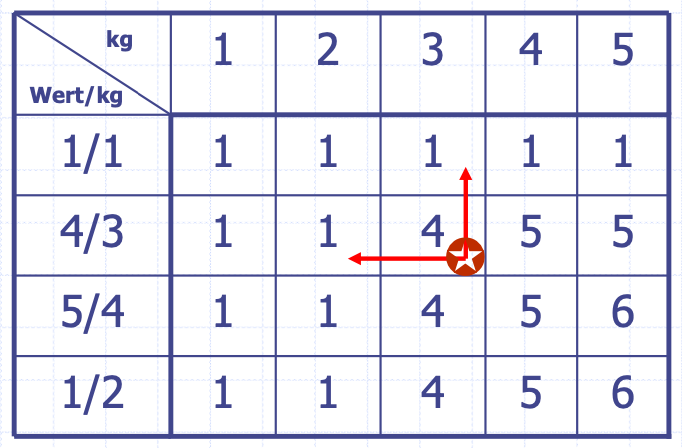
\includegraphics[scale=.2]{graphic/10 DynamicProgramming/Dynamische Programmierung.png}
    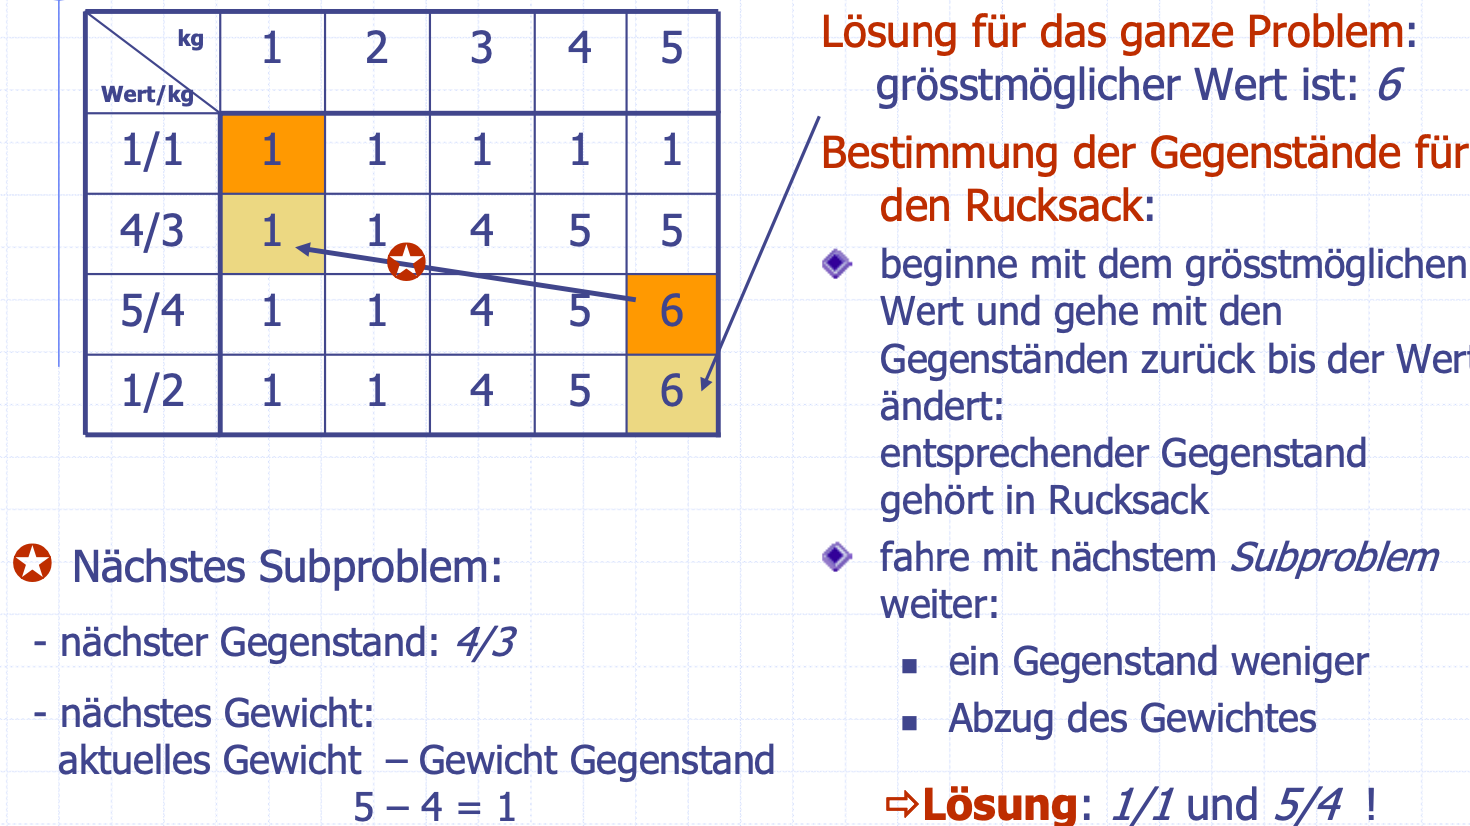
\includegraphics[scale=.2]{graphic/10 DynamicProgramming/Dynamische Programmierung2.png}
\end{center}
\vspace{-8pt}

\subsection{Technik der dynamischen Programmierung}
\begin{itemize}
    \item Anwendbar auf Probleme welche anfänglich sehr grosse Laufzeit zu benötigen
    \item Voraussetzung:
    \begin{itemize}
        \item \textbf{Einfache Subprobleme:} Subprobleme können durch wenigen Variablen ausgedrückt werden
        \item \textbf{Subproblem-Optimierung:} globale Optimum kann durch optimale Subprobleme ausgedrückt werden
        \item \textbf{Subprobleme überlappen: }Subprobleme sind nicht unabhängig, sie überlappen
    \end{itemize}
\end{itemize}

\subsection{Subsequenzen}
\begin{itemize}
    \item Nicht dasselbe wie ein Substring
    \item Beispiel: ABCDEFGHIJK
    \begin{itemize}
        \item Subsequenz: ACEGIJK
        \item Subsequenz: DFGHK
        \item Nicht Subsequenz: DAGH
    \end{itemize}
\end{itemize}

\subsection{Längste gemeinsame Subsequenz (LCS)}
\begin{itemize}
    \item Gegeben die beiden Strings X und Y
    \item finde die längste Subsequenz welche in X sowie auch in Y enthalten ist
    \item Beispiel: ABCDEFG und XZACKDFWGH haben ACDFG als längste gem. SubSeq.
\end{itemize}
\subsubsection{Brute-Force}
\begin{itemize}
    \item Aufzählung aller Subsequenzen von X
    \item Testen welche ebenfalls Subsequenzen von Y sind
    \item längste Subsequenz als Resultat wählen
    \item exponentieller Algorithmus! $\rightarrow$ $O(n^2)$
\end{itemize}
\subsubsection{dynamischer Programmierung}
\begin{itemize}
    \item Definiere L[i,j] als Länge der längsten gemeinsamen Subsequenz von X[0..i] and Y[0..j]
    \item Erlaube -1 als Index, so dass L[-1,k] = 0 and L[k,-1]=0
    \item Definiere L[i,j] folgendermassen:
    \begin{itemize}
        \item wenn $xi = yj$, dann L[i,j] = L[i-1,j-1] + 1 (Übereinstimmung)
        \item wenn $xi \neq yj$, dann L[i,j] = max{L[i-1,j], L[i,j-1]} (keine Übereinstimmung)
    \end{itemize}
\end{itemize}
\vspace{-8pt}
\begin{center}
    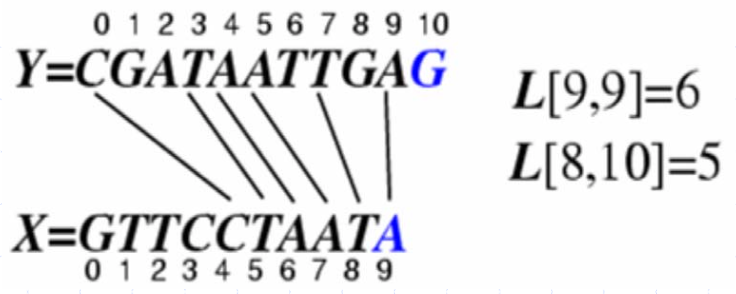
\includegraphics[scale=.2]{graphic/10 DynamicProgramming/Versuch mit dynamischer Programmierung.png}
    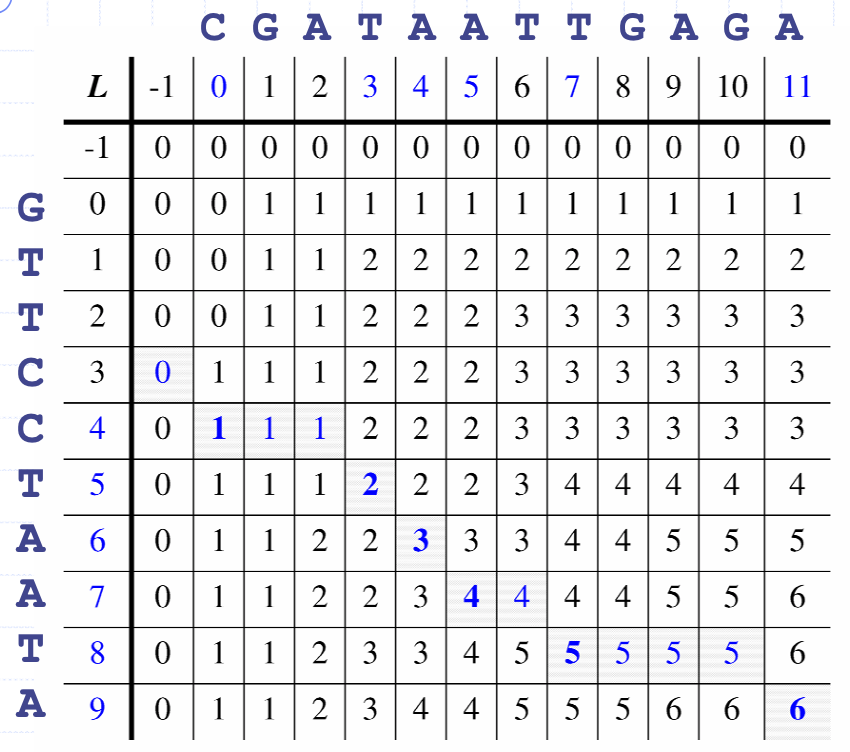
\includegraphics[scale=.2]{graphic/10 DynamicProgramming/Versuch mit dynamischer Programmierung2.png}
\end{center}
\vspace{-8pt}

\begin{lstlisting}
Algorithmus LCS(X,Y):
    Input: Strings X,Y with n,m Elements
    Output: array L[i,j]
    for i=1 to n-1 do
        L[i,-1] = 0
    for j=0 to m-1 do
        L[-1, j] = 0
    for i=0 to n-1 do
        for j=0 to m-1 do
            if x_i = y_i then
                L[i,j] = L[i-1, j-1] + 1
            elseL[i,j] = max{L[i-1,j],L[i,j-1]}
    return array L
\end{lstlisting}

\subsubsection{Laufzeit}
\begin{itemize}
    \item äusserer Loop iteriert n mal
    \item innerer Loop iteriert m mal
    \item konstanter Aufwand innerhalb jeder Iteration des inneren Loops
    \item Somit ist die totale Laufzeit: O(nm)
\end{itemize}

\subsubsection{Auslesen der LCS}
\begin{center}
    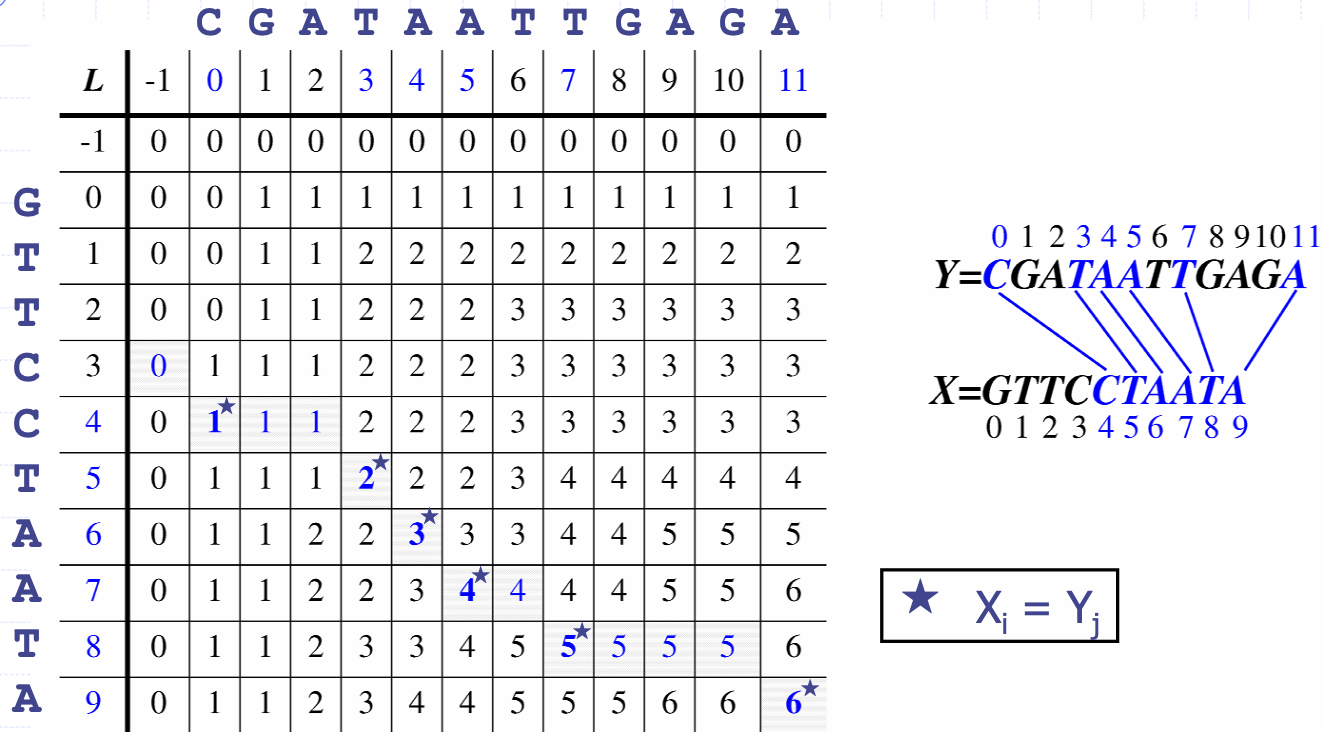
\includegraphics[scale=.2]{graphic/10 DynamicProgramming/Auslesen der LCS.png}
\end{center}

\newpage